\documentclass[sigplan,screen]{acmart}

\usepackage{algorithm}
\usepackage{algpseudocode}
\usepackage{color}
\usepackage{xcolor}
\usepackage{float}
\usepackage{subfig}

\AtBeginDocument{%
  \providecommand\BibTeX{{%
    \normalfont B\kern-0.5em{\scshape i\kern-0.25em b}\kern-0.8em\TeX}}}

\citestyle{acmauthoryear}

\begin{document}
\title{Particle Based Fluids in Rust}

\author{Luka Mijalkovic}
\email{luka.mijalkovic@mail.utoronto.ca}
\affiliation{%
  \institution{University of Toronto}
  \streetaddress{27 King's College Circle}
  \city{Toronto}
  \state{Ontario}
  \country{Canada}
}

\renewcommand{\shortauthors}{Luka Mijalkovic}

\acmConference[CSC417 '21]{Algorithm Implementations}{December 2021}{Toronto, ON, Canada}

\begin{CCSXML}
<ccs2012>
   <concept>
       <concept_id>10010147.10010371.10010352.10010379</concept_id>
       <concept_desc>Computing methodologies~Physical simulation</concept_desc>
       <concept_significance>500</concept_significance>
       </concept>
 </ccs2012>
\end{CCSXML}

\ccsdesc[500]{Computing methodologies~Physical simulation}

\keywords{fluid simulation, SPH, rustlang, constraint fluids, position based dynamics}

\begin{teaserfigure}
  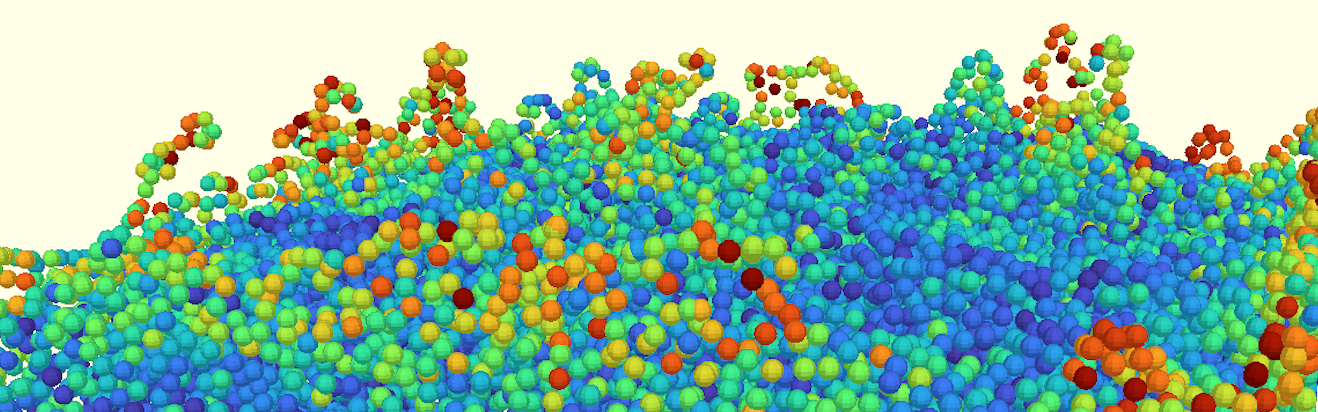
\includegraphics[width=\textwidth]{images/teaser.png}
  \caption{4000 active particles, method from \cite{Muller}}
  \Description{Multi-threaded algorithm run with 4000 particles. Octree used for nearest neighbor search.}
  \label{fig:teaser}
\end{teaserfigure}

\settopmatter{printacmref=false} % Removes citation information below abstract
\renewcommand\footnotetextcopyrightpermission[1]{} % removes footnote with conference information in first column
\pagestyle{plain} % removes running headers

\maketitle

\section{Introduction}
In their paper ``Position Based Fluids'', \cite{Muller} present a constraint based approach to model fluids. They begin by introducing a constraint equation obtained from \cite{Bodin} involving neighboring particles in a fluid simulation. From there, they explain the piecewise development of a constraint gradient initially given by \cite{Monaghan1992}, of which they use to perform a series of Newton steps along the gradient each integration time step.

In this implementation, I make use of the Rust library \href{https://docs.rs/rayon/latest/rayon/}{\texttt{rayon}} when parallelizing the algorithm, allowing it to utilize multiple CPU threads. Additionally, I make use of an octree data structure to speed up the particle neighbor search. Finally, I decouple the rendering and physics threads to allow for smoother previewing. This is all in done in contrast to \cite{Muller}, who develop their algorthm to run on the GPU through use of NVIDIA's proprietary \texttt{CUDA} architecture. Hence, while my implementation is not as efficient it is far easier to implement, requiring less boilerplate code and no GPU kernels.

\section{Constraints}
\subsection{Constraint Function}
Fundamentally, the algorithm by \cite{Muller} works by enforcing a constraint equation on each of the particles. Originally from \cite{Bodin}, they define a \textit{density constraint function}, $C_i$, for the $i^{th}$ particle as follows:
\begin{equation}
  C_i(\textbf{p}_1, ... , \textbf{p}_n) = \frac{\sum_j W(\textbf{p}_i - \textbf{p}_j, h)}{\rho_0} - 1
\end{equation}
The inputs, $\textbf{p}_1, ..., \textbf{p}_n$, are the $n$ positions of all particles neighboring the $i^{th}$ particle within some radius $r$. The variable $\rho_0$ represents the rest density of the fluid. The summation in the numerator is often denoted $\rho_i$, and it is known as the \textit{standard SPH density estimator} for a particle. The summation goes over the $n$ particles in the input, $\textbf{p}_1, ..., \textbf{p}_n$.

$W(\vec{\mathbf{v}}, h)$ is a function that takes in an $n$ dimensional vector, $\vec{\mathbf{v}}$, a unit distance, $h$, and returns a scalar of $\mathbb{R}^{\geq 0}$. It is discussed in more detail in \ref{sec:kernel_functions}.

\subsection{Constraint Function Gradient}
With the constraint function $C_i$ well defined, we can now establish its gradient with respect to any input particle $\textbf{p}_k$, where $1 \leq k \leq n$. Borrowing notation from \cite{Muller}, this is denoted as $\nabla_{\mathbf{p}_k} C_i$. The original equation is derived from \cite{Monaghan1992}, after which \cite{Muller} have provided a piecewise definition like so:
\begin{equation}
  \nabla_{\mathbf{p}_k} C_i = \frac{1}{\rho_0} \begin{cases}
    \sum_j \nabla_{\mathbf{p}_i} W(\mathbf{p}_i - \mathbf{p}_j, h) & k = i\\
    -\nabla_{\mathbf{p}_k} W(\mathbf{p}_i - \mathbf{p}_k, h) & k \neq i
  \end{cases}
\end{equation}
I have adopted  my own notation to clarify some ambiguity in the definition. Again, the summation is only over neighboring particles of particle $i$.

\subsection{Constraint Equation}
Using the constraint function $C_i$ and its gradient $\nabla_{\mathbf{p_k}} C_i$ we can develop the most important equation given by \cite{Muller}. By trying to enforce uniform density for every single particle, we can make the following equation hold for all particles:
\begin{equation}
  C_i(\mathbf{p}_1 + \Delta \mathbf{p}_1, ...,\mathbf{p}_n + \Delta \mathbf{p}_n) = 0
\end{equation}
\label{constraint_eq}
From here, they develop the following first order approximation:
\begin{align}
  0 &= C_i(\mathbf{p}_1 + \Delta \mathbf{p}_1, ...,\mathbf{p}_n + \Delta \mathbf{p}_n)\\
  &\approx C_i(\mathbf{p}_1, ...,\mathbf{p}_n) + \sum_j (\nabla_{\mathbf{p}_j} C_i)^\top \Delta \mathbf{p}_j\\
  &\approx C_i(\mathbf{p}_1, ...,\mathbf{p}_n) + \sum_j (\nabla_{\mathbf{p}_j} C_i)^\top \nabla_{\mathbf{p}_j} C_i \lambda_i
\end{align}
Where $\lambda_i$ is some arbitrarily small scalar value that will be solved for.
\label{constraint_approx}

\section{Finding $\lambda$ and $\Delta \textbf{p}$}
\subsection{Deriving $\lambda$}
Given Equation (\hyperref[constraint_approx]{6}), we can derive an equation for $\lambda_i$ like so:
\begin{align}
  0 &\approx C_i(\mathbf{p}_1, ...,\mathbf{p}_n) + \sum_j (\nabla_{\mathbf{p}_j} C_i)^\top \nabla_{\mathbf{p}_j} C_i \lambda_i\\
  - \sum_j (\nabla_{\mathbf{p}_j} C_i)^\top \nabla_{\mathbf{p}_j} C_i \lambda_i &\approx C_i(\mathbf{p}_1, ...,\mathbf{p}_n)\\
  \lambda_i &\approx - \frac{C_i(\mathbf{p}_1, ...,\mathbf{p}_n)}{\sum_j (\nabla_{\mathbf{p}_j} C_i)^\top \nabla_{\mathbf{p}_j} C_i}\\
  \lambda_i &\approx - \frac{C_i(\mathbf{p}_1, ...,\mathbf{p}_n)}{\sum_j ||\nabla_{\mathbf{p}_j} C_i||^2}
\end{align}
\subsection{Relaxation Constant $\mathcal{E}$}
Notice that Equation (\hyperref[constraint_approx]{10}) will cause numerical issues when the denominator is close to 0. Hence, \cite{Muller} suggest a \textit{relaxation parameter}, $\mathcal{E}$. A concept introduced by \cite{Solenthaler} which will ensure this never occurs:
\begin{equation}
  \lambda_i \approx - \frac{C_i(\mathbf{p}_1, ...,\mathbf{p}_n)}{\sum_j ||\nabla_{\mathbf{p}_j} C_i||^2 + \mathcal{E}}
\end{equation}
\subsection{Assembling $\Delta \mathbf{p}$}
From here, \cite{Muller} derived an approximation for $\Delta \mathbf{p}_i$ by assembling all $\lambda$ values like so:
\begin{equation}
  \Delta \mathbf{p}_i \approx \frac{1}{\rho_0} \sum_j (\lambda_i + \lambda_j) \nabla_{\mathbf{p}_i}W(\mathbf{p}_i - \mathbf{p}_j, h)
\end{equation}
At this point, the algorithm is functionally finished. With an appropriate time integration scheme, the simulation can be run using $\Delta \mathbf{p}$ updates. The terms introduced in \ref{sec:stability_corrections} are mostly just visual effects.

\section{Stability and Realism}
\label{sec:stability_corrections}

\subsection{Artificial Pressure}

As noted by \cite{Muller}, when a particle is left with little neighbors it will struggle to reach rest density. Hence, they follow the method of \cite{Monaghan2000} by adding a constant, $s_{\text{corr}}$, to account for this:
\begin{equation}
  \Delta \mathbf{p}_i \approx \frac{1}{\rho_0} \sum_j (\lambda_i + \lambda_j + s_{\text{corr}}) \nabla_{\mathbf{p}_i}W(\mathbf{p}_i - \mathbf{p}_j, h)
\end{equation}
Where $s_{\text{corr}}$ is defined as:
\begin{equation}
  s_{\text{corr}} = -k \left( \frac{W(\mathbf{p}_i - \mathbf{p}_j, h)}{W(\Delta \mathbf{q}, h)} \right)^n
\end{equation}
This boosts surface tension of the fluid. The values recommended were $k = 0.1$, $n = 4$, and $\Delta \mathbf{q}$ as a vector with magnitude in the interval $[0.1h, 0.3h]$.

\subsection{Vorticity}
In order to reduce energy loss caused by damping in position based methods, \cite{Muller} use vorticity confinement. This is done by calculating the vorticity for each particle. For the proceeding equations, $m$ is the number of neighbors:
\begin{equation}
  \boldsymbol{\omega}_i = \begin{cases} 
    \sum_j \mathbf{v}_{ij} \times \nabla_{p_j} W(\mathbf{p}_i - \mathbf{p}_j, h) & m > 0\\
    \vec{0} & m = 0
  \end{cases}
\end{equation}
From here, a \textit{location vector}, $\mathbf{N}_i$, is defined:
\begin{equation}
  \mathbf{N}_i = \begin{cases}
    \frac{\nabla | \boldsymbol{\omega}_i |}{|\nabla | \boldsymbol{\omega}_i ||} & |\nabla | \boldsymbol{\omega}_i || > 0\text{ and }m > 0\\
    \vec{0} & \text{otherwise}
    \end{cases}
\end{equation}
Finally, a vorticity force, $\mathbf{f}_i^{\text{vort}}$, can be calculated using $\mathbf{N}_i$ and $\mathbf{\omega}_i$:
\begin{equation}
  \mathbf{f}_i^{\text{vort}} = \epsilon (\mathbf{N}_i \times \boldsymbol{\omega}_i)
\end{equation}
Where $\epsilon$ is a small scalar which can be tuned.
\subsection{Viscosity}
Additionally, \cite{Muller} add a simple XSPH viscosity correction step from \cite{Schechter}:
\begin{equation}
  \mathbf{v}_i^{\text{visc}} = \mathbf{v}_i + c \sum_j \mathbf{v}_{ij} W(\mathbf{p}_i - \mathbf{p}_j, h)
\end{equation}

\section{Algorithm}
\subsection{Pseudocode}
The implementation I used was 1:1 with that which was written by \cite{Muller}. However, as this one is CPU based I have notated where the thread spawning/joining must occur.
\begin{algorithm}
\caption{CPU Multithreaded Position Based Fluids}
\label{alg:cpu}
\begin{algorithmic}[1]
  \State{\texttt{spawn\_assign\_k\_threads(particles)}} \Comment{Split work}
  \ForAll{particles assigned in thread $k$}
    \State $\mathbf{v}_i^{t+1} \gets \mathbf{v}_i^t + \Delta t \mathbf{f}_i^{\text{ext}}$
    \State $\mathbf{p}_i^{t+1} \gets \mathbf{p}_i^t + \Delta t \mathbf{v}_i^{t+1}$
  \EndFor
  \State \texttt{join\_threads()} \Comment{Combine all particle calculations}
  \State{\texttt{neighbor\_search(particles)}} \Comment{Varies on search}
  \ForAll{solver iteration $q$}
    \State{\texttt{spawn\_assign\_k\_threads(particles)}}
    \ForAll{particles assigned in thread $k$}
      \State $\lambda^q_i \gets - \frac{C_i(\mathbf{p}^{t+1}_1, ...,\mathbf{p}^{t+1}_n)}{\sum_j ||\nabla_{\mathbf{p}^q_j} C_i||^2 + \mathcal{E}}$
    \EndFor
    \State \texttt{join\_threads()}
    \State{\texttt{spawn\_assign\_k\_threads(particles)}}
    \ForAll{particles assigned in thread $k$}
      \State $\Delta \mathbf{p}^q_i \gets \frac{1}{\rho_0} \sum_j (\lambda^q_i + \lambda^q_j) \nabla_{\mathbf{p}^{t+1}_i}W(\mathbf{p}^{t+1}_i - \mathbf{p}^q_j, h)$
      \State{\texttt{collision\_response()}}
      \State $\mathbf{p}_i^{t+1} \gets \mathbf{p}_i^{t+1} + \Delta \mathbf{p}^q_i$
    \EndFor
    \State \texttt{join\_threads()}
  \EndFor
  \State{\texttt{spawn\_assign\_k\_threads(particles)}}
  \ForAll{particles assigned in thread $k$}
    \State $\mathbf{v}_i \gets \frac{1}{\Delta t} \left( \mathbf{p}^{t+1}_i - \mathbf{p}^t_i\right)$
  \EndFor
  \State \texttt{join\_threads()}
  \State{\texttt{apply\_vorticity()}} \Comment{Use $\mathbf{p}^{t+1}$ not $\mathbf{p}^t$}
  \State{\texttt{apply\_viscosity()}} \Comment{Use $\mathbf{v}^{t+1}$ not $\mathbf{v}^t$}
\end{algorithmic}
\end{algorithm}

\section{Benchmarks}
\label{sec:benchmarks}
\subsection{Neighbor Search}
For the neighbor search (each run through of \hyperref[alg:cpu]{Algorithm 1}, line 7), I tested two algorithms. The first was a classic $\mathcal{O}(n^2)$ search, in which I checked for every particle $i$, if another particle $j$ was within radius $r$. This proved to be very inefficient and greatly slowed down the algorithm. When multithreading this algorithm, the performance actually went down, as can be seen in \hyperref[tab:runtimes]{Table 1}. I have a suspicion this has to do with CPU cache misses \cite{Meyers} due to how the data was aligned, but I can't say for certain. Regardless, it wasn't very fast so I didn't see much of a need to intensely profile it. Rather, I just opted for a faster data structure to query points, an octree.

As suggested by \cite{Muller}, I also dynamically generated an octree each run through in order to query neighbor points. I made use of the open source Rust library \href{https://docs.rs/octree/latest/octree/}{\texttt{octree}} to instantiate the data structure. After creating the octree I queried for the neighbors of all points, using both a multithreaded and a single-threaded query. As can be seen in \hyperref[tab:runtimes]{Table 1}, the performance seen when multithreading the point querying gave a big improvement of 250\%. This in stark contrast to the naive algorithm which performed approximately 10\% worse multithreaded.

\begin{table}
  \caption{Runtime of differing neighbor search algorithms, 95\% confidence interval. Tested with 5,000 particles on a 13" 2016 Macbook Pro, measured using \href{https://docs.rs/criterion/latest/criterion/}{\texttt{criterion}}}
  \label{tab:runtimes}
  \begin{tabular}{c|ccc}
    \toprule
    Algorithm &Lower (ms) &Mean (ms) &Upper (ms)\\
    \midrule
    Naive, Single-threaded &92.423 &93.320 &94.345\\
    Naive, Multi-threaded &101.67 &102.34 &103.06\\
    Octree, Single-threaded &50.293 &50.646 &51.030\\
    Octree, Multi-threaded &20.092 &20.318 &20.613\\
  \bottomrule
\end{tabular}
\end{table}

\subsection{Flamegraphs}

\begin{figure}[H]
  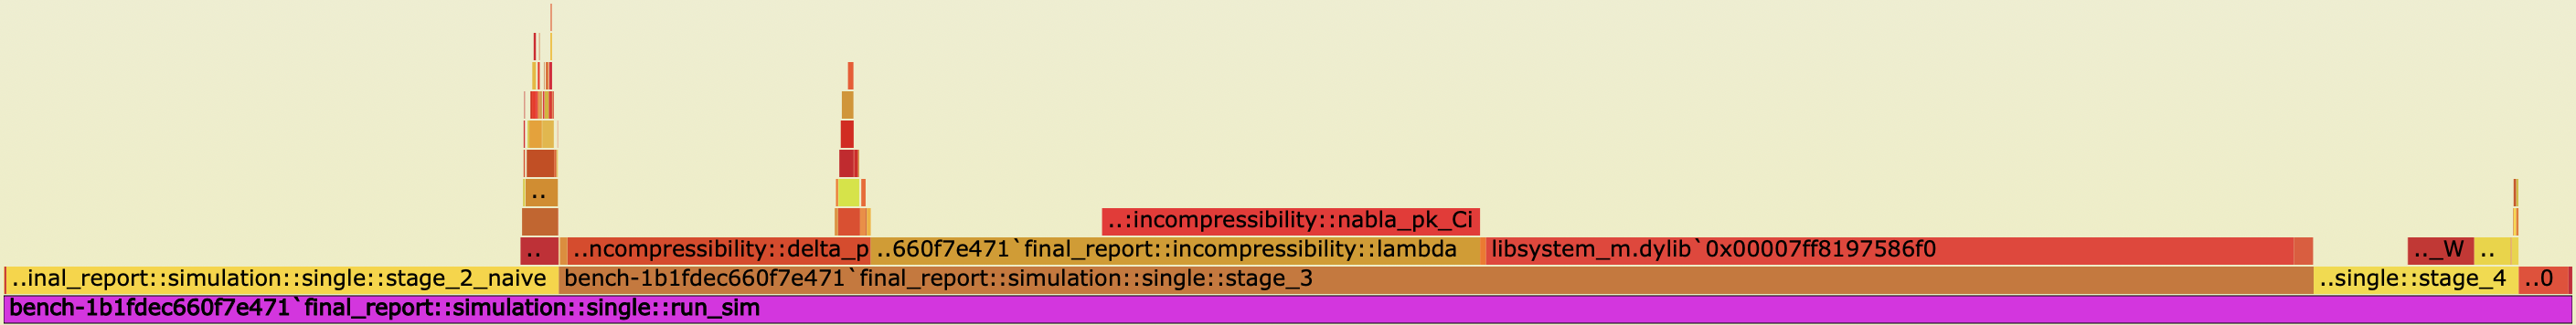
\includegraphics[width=\columnwidth]{images/single_naive_flamegraph.png}
  \caption{Flamegraph of performance using the single-thread implementation with naive search. Tested with 5,000 particles.}
  \label{fig:single_naive_flamegraph}
\end{figure}

\begin{figure}[H]
  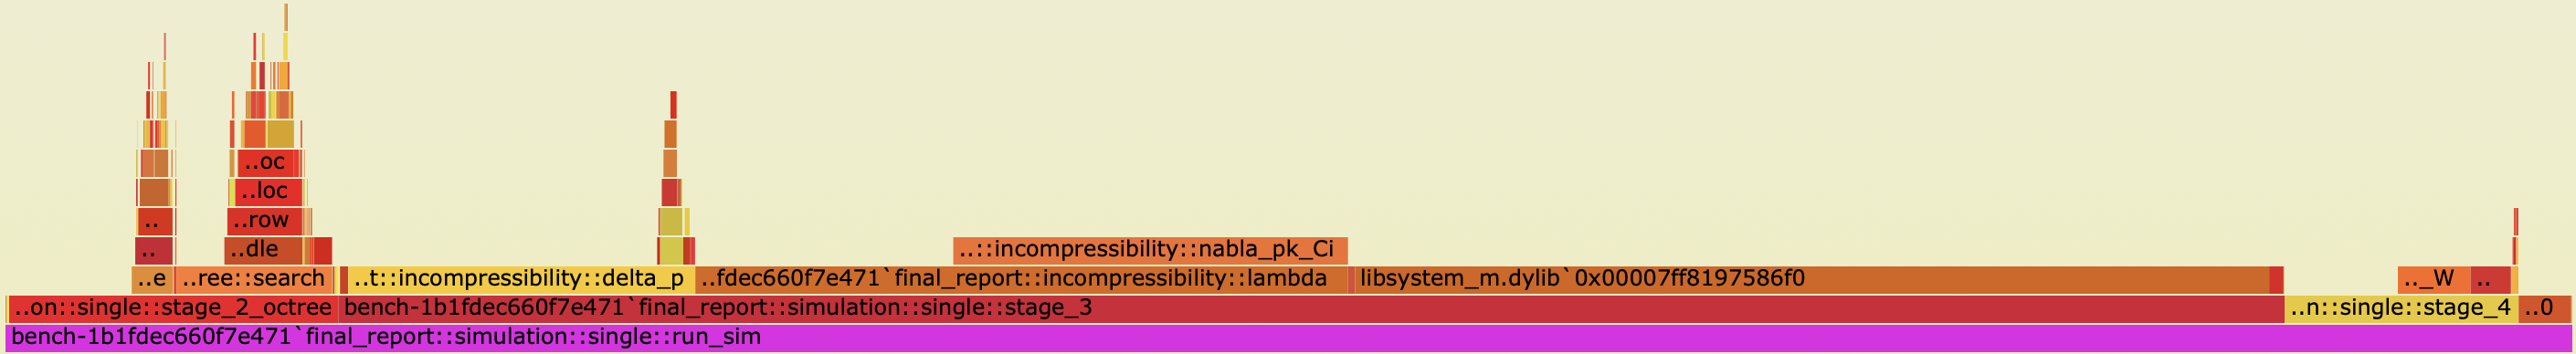
\includegraphics[width=\columnwidth]{images/single_octree_flamegraph.png}
  \caption{Flamegraph of performance using the single-thread implementation with octree search. Tested with 5,000 particles.}
  \label{fig:single_octree_flamegraph}
\end{figure}

In order to create flamegraphs of the algorithm, I disabled function inlining by leaving \texttt{[inline(never)]} above the important sections and ran it on the single-threaded version. This yielded flamegraphs \hyperref[fig:single_naive_flamegraph]{Figure 2} and \hyperref[fig:single_octree_flamegraph]{Figure 3}.

As one can see by the flamegraphs, octree performance is indeed better than naive for the single threaded version. Experimentally it is very close to the isolated benchmarks from \hyperref[tab:runtimes]{Table 1}. It is also evident that a large amount of time was spent calculating both $\lambda_i^q$ and $\Delta \mathbf{p}_i^q$ on lines 11 and 16 of \hyperref[alg:cpu]{Algorithm 1}. This makes sense because they are indeed heavy summations.

Interestingly, the algorithm seemed to spend roughly half the time querying the octree, and the other half building.

Creating flamegraphs for the multi-threaded implementation was not practical because \texttt{rayon} muddles the call stack when thread switching.

\subsection{Overall}

\begin{figure}
  \centering
  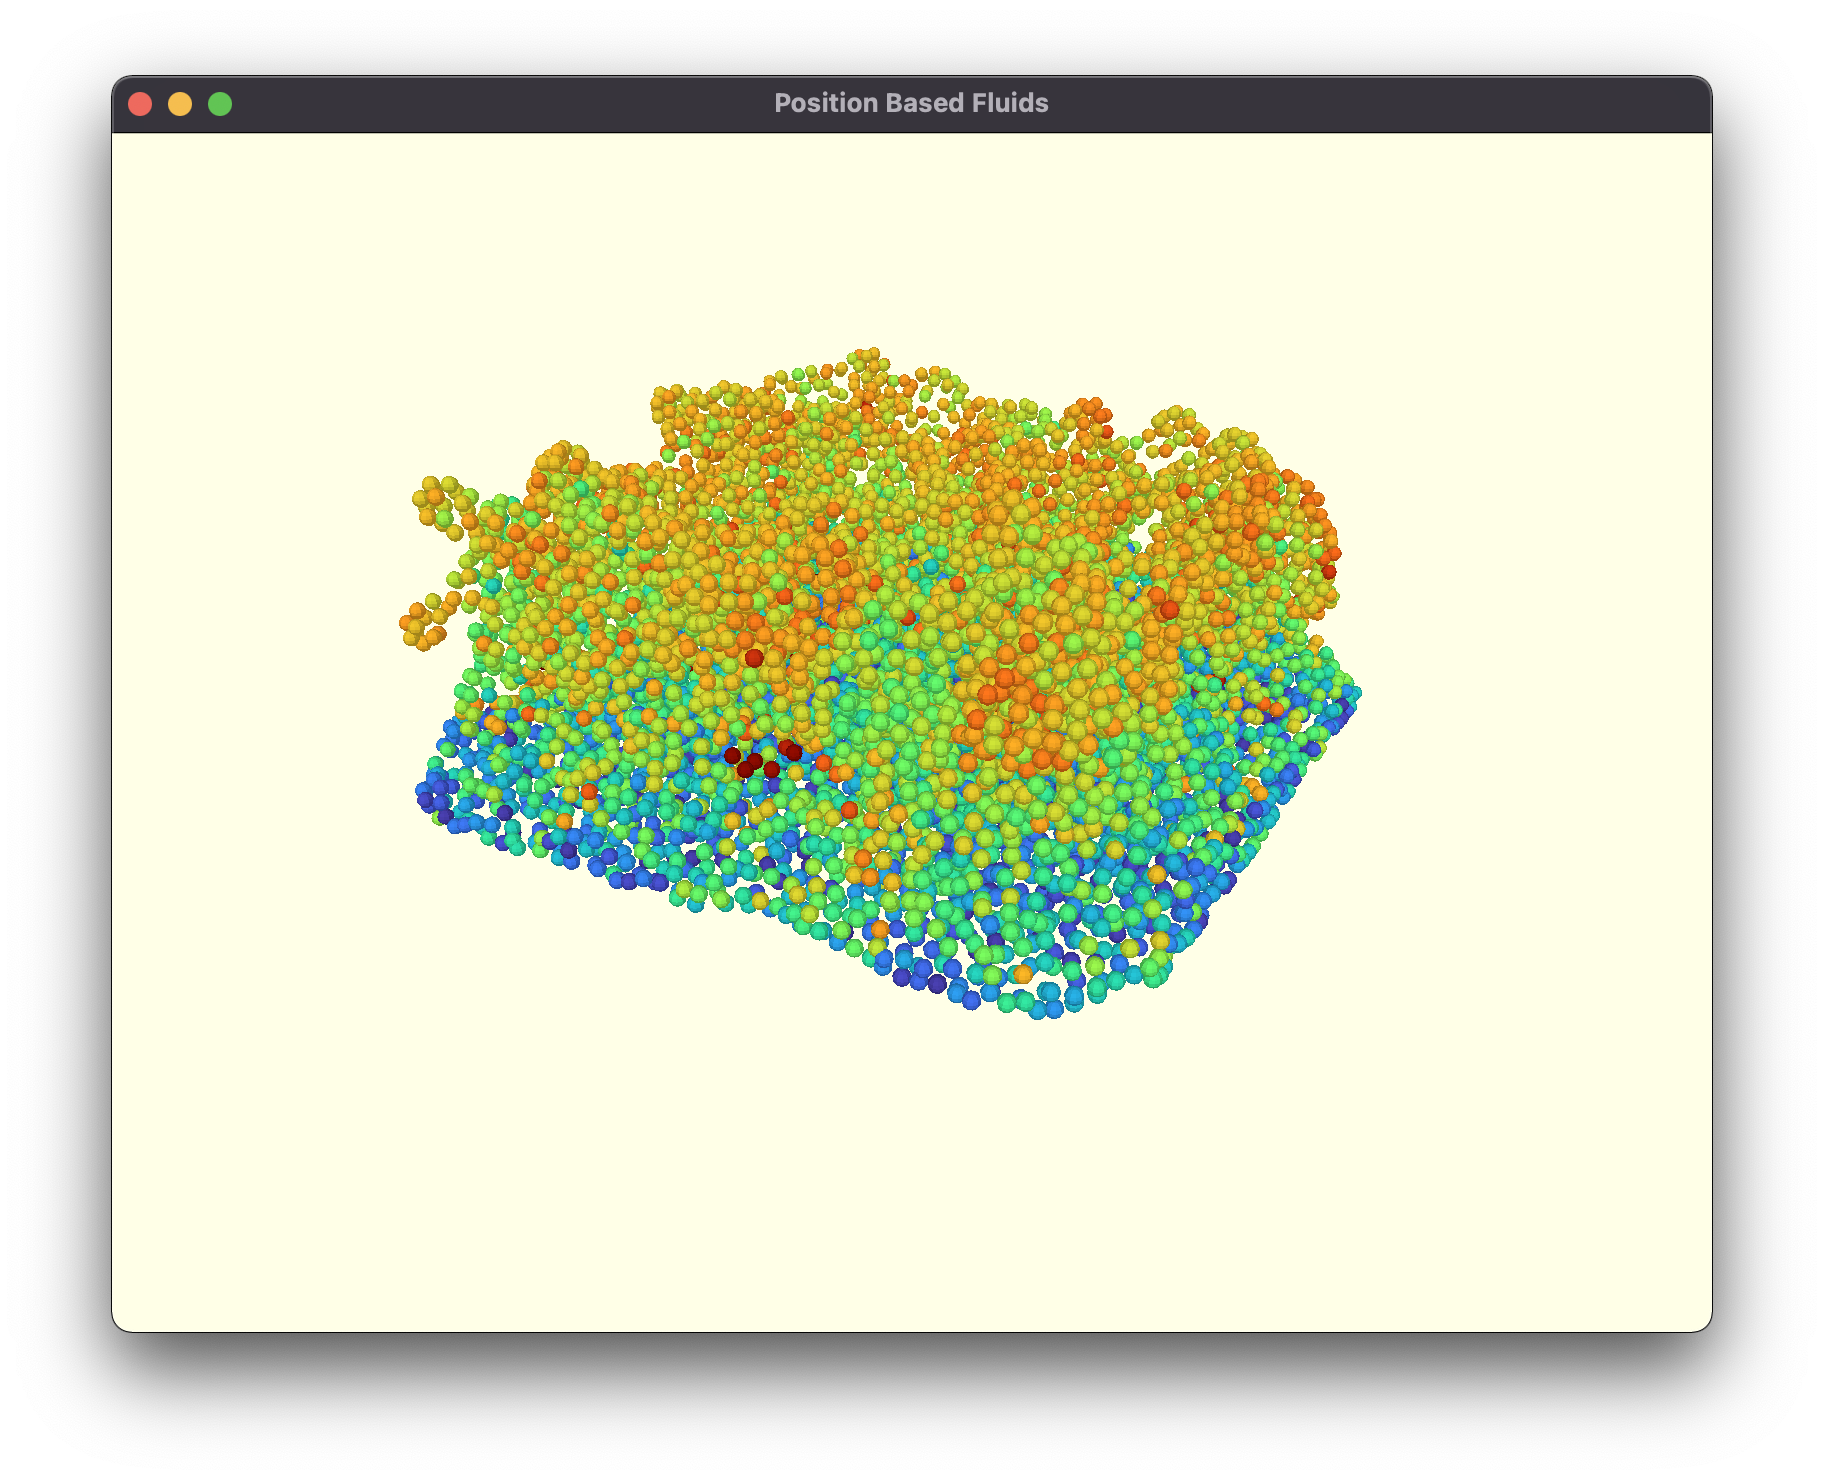
\includegraphics[width=\columnwidth]{images/simulation_start.png} \label{fig:sim_start}
  \vspace{0.00mm} 
  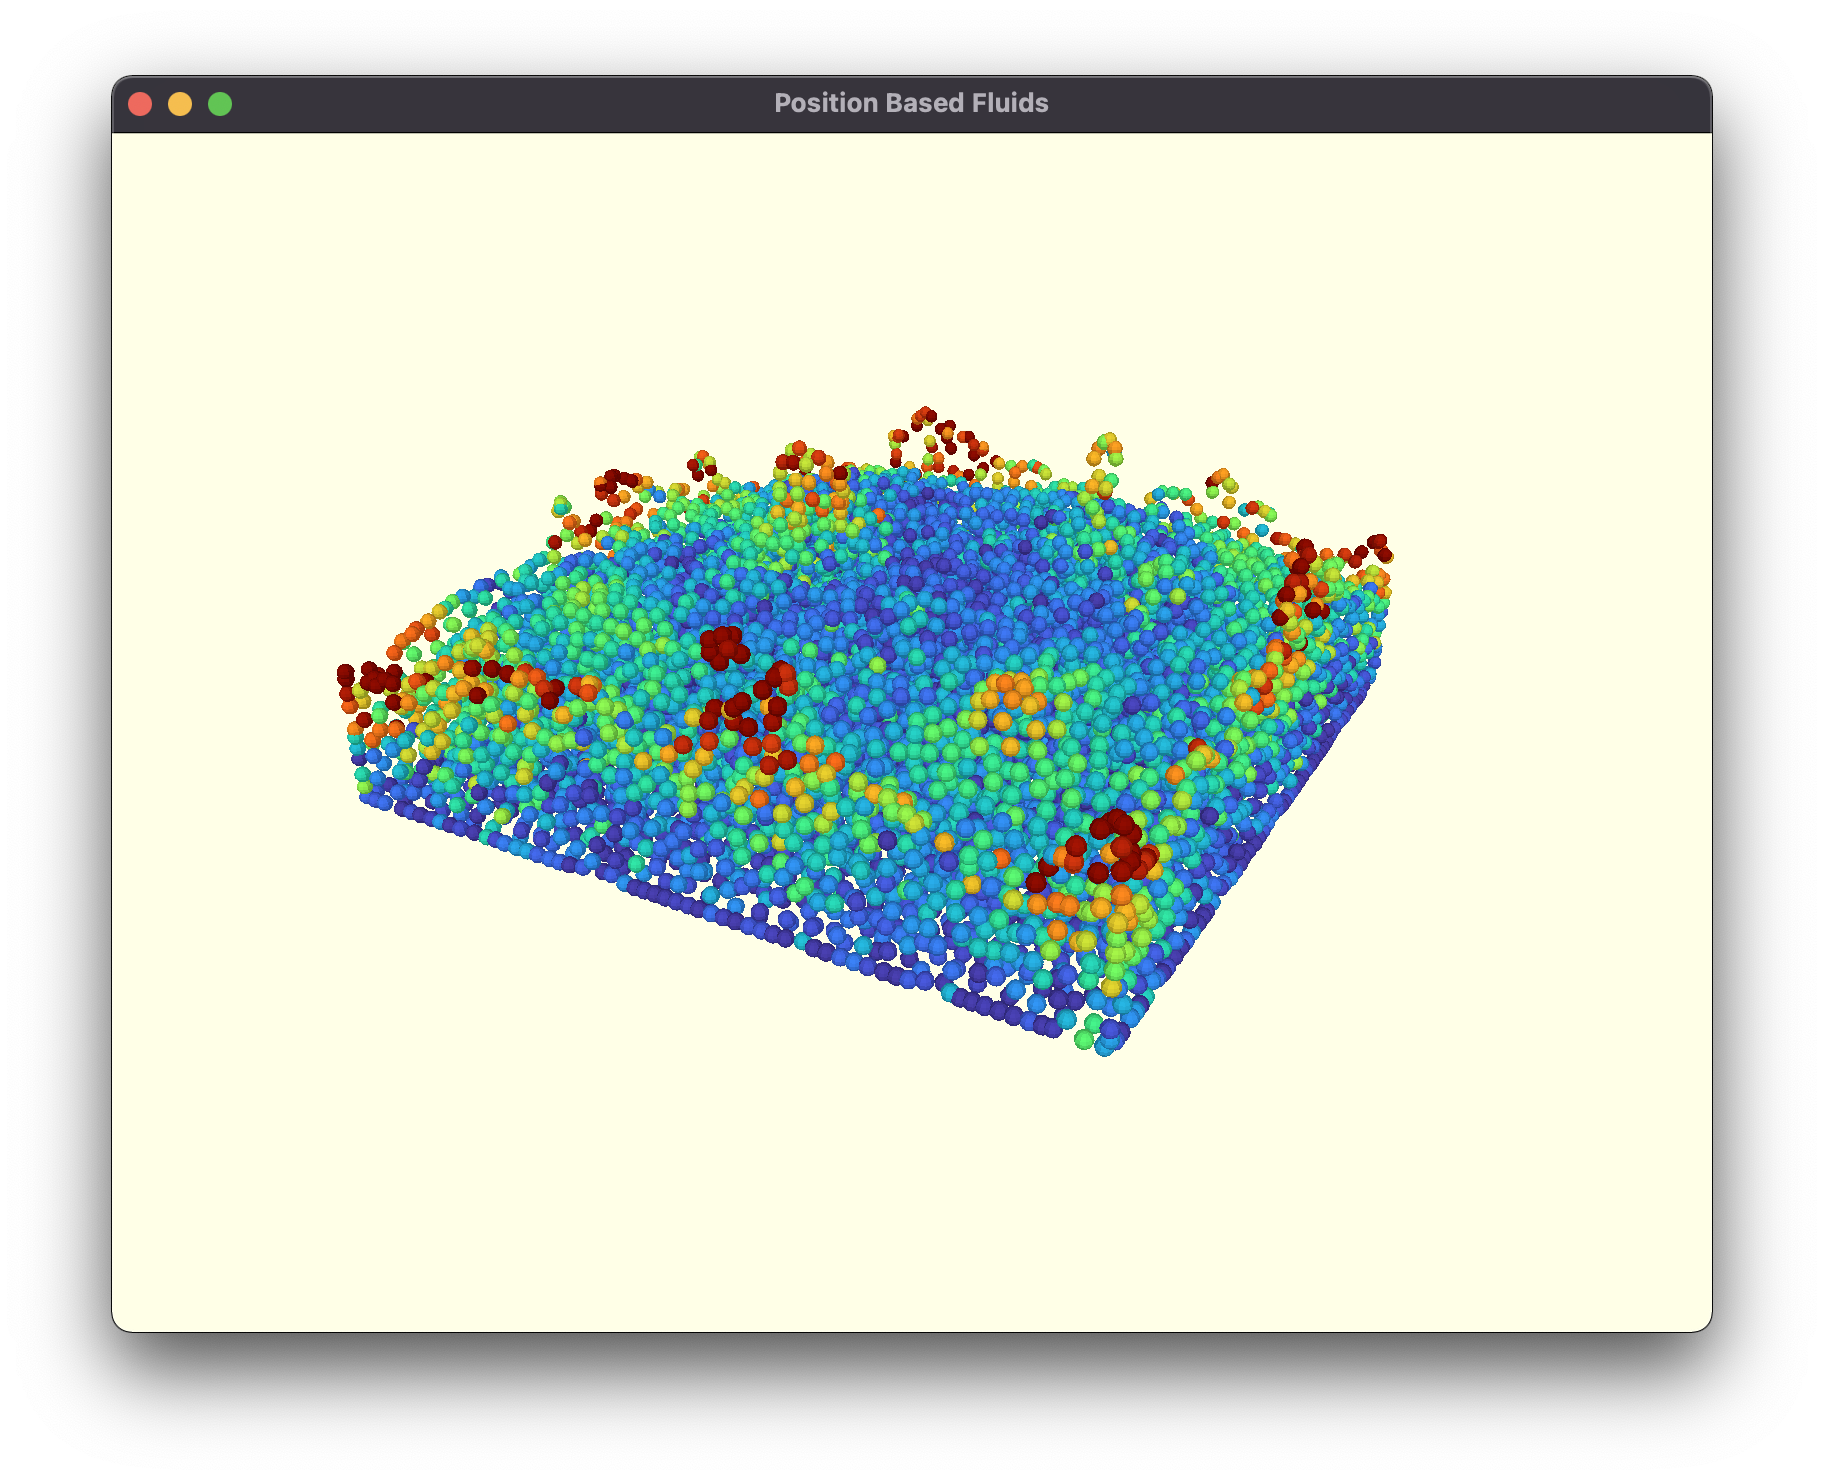
\includegraphics[width=\columnwidth]{images/simulation_middle.png} \label{fig:sim_middle}
  \vspace{0.00mm} 
  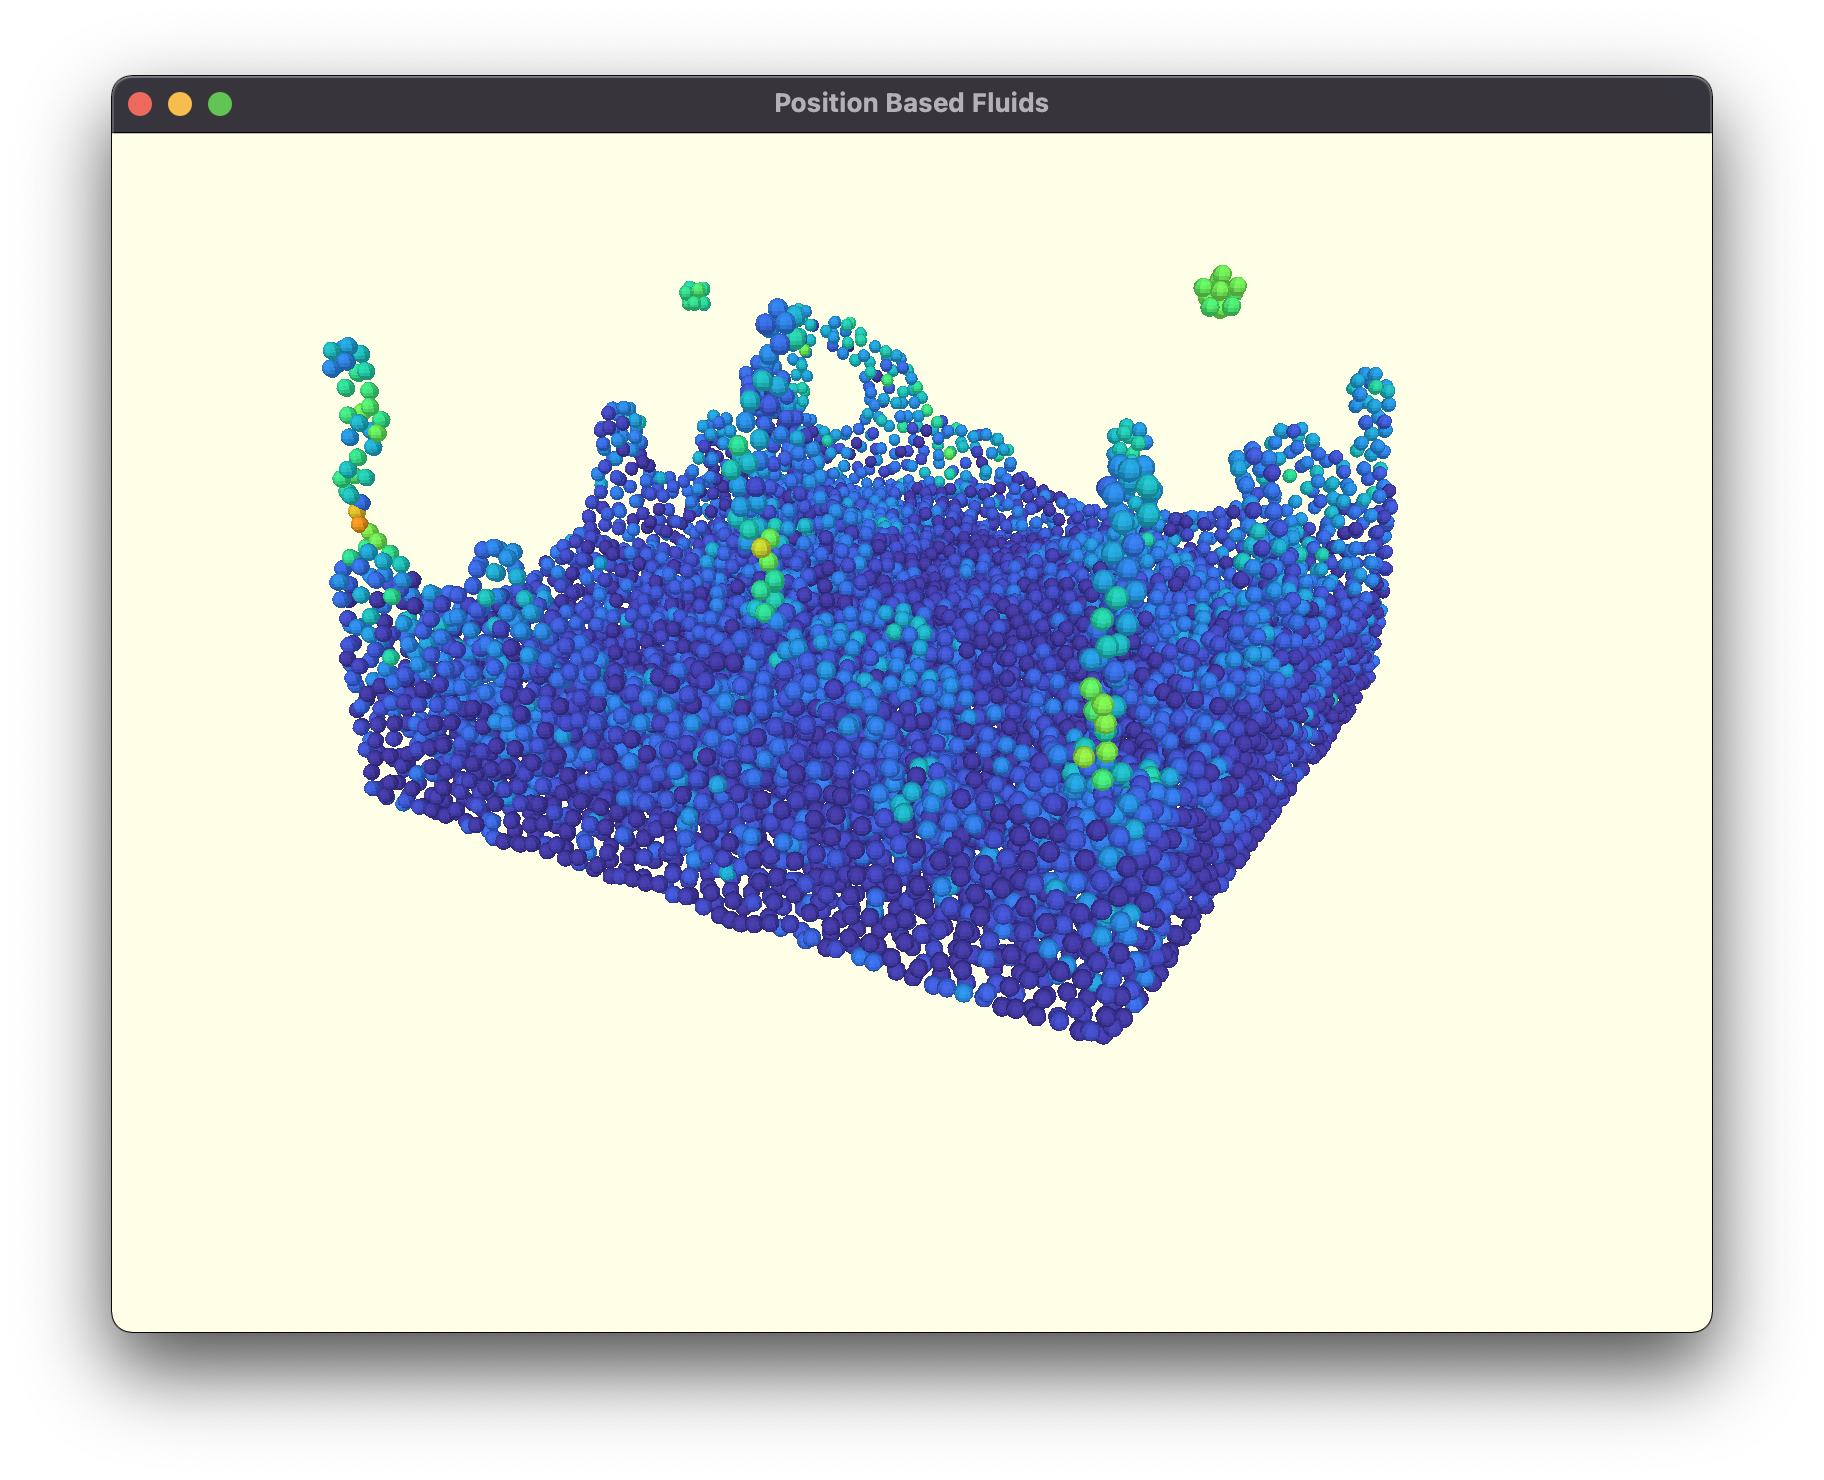
\includegraphics[width=\columnwidth]{images/simulation_end.png} \label{fig:sim_end}
  \caption{Progression of a simulation with 10,000 particles}
\end{figure}

\begin{table}[H]
  \caption{Average simulation step time using differing setups, 95\% confidence interval. Tested with 5,000 particles and 3 solver iterations.}
  \label{tab:sim_runtimes}
  \begin{tabular}{c|ccc}
    \toprule
    Algorithm &Lower (ms) &Mean (ms) &Upper (ms)\\
    \midrule
    Naive, Single-threaded &424.65 &426.67 &429.17\\
    Naive, Multi-threaded &218.29 &219.75 &221.44\\
    Octree, Single-threaded &369.56 &370.84 &372.41\\
    Octree, Multi-threaded &139.78 &140.73 &142.00\\
  \bottomrule
\end{tabular}
\end{table}

I additionally ran \href{https://docs.rs/criterion/latest/criterion/}{\texttt{criterion}} on the average runtime of an entire simulation step. This was done with randomly generated locations each time, and the results can be found in \hyperref[tab:sim_runtimes]{Table 2}. It might seem like this table contradicts \hyperref[tab:sim_runtimes]{Table 2} due to higher performance with the multithreaded naive search, however this multithreading was not limited to the search algorithm. Every line spawning threads in \hyperref[alg:cpu]{Algorithm 1} was executed, thus the overall speed up triumphed the worse search algorithm. 

The octree search with a multithreaded implementation performed the best overall, as was expected. Steps were calculated roughly 300\% faster than the single threaded naive implementation. All testing was performed on a 13 inch Macbook Pro 2016.

\section{Rendering}

In order to render particles I made use of \href{https://docs.rs/glium/latest/glium/}{\texttt{glium}}, a memory safe wrapper around \texttt{OpenGL}. Batch rendering was performed to reduce the amount of VAO binding required. This allowed for thousands of particles to barely affect the GPU rendering times.

\section{Conclusions}

Due to ease of use with \href{https://docs.rs/rayon/latest/rayon/}{\texttt{rayon}}, parallelizing the code was relatively straight forward. It mostly consisted of changing top level iterators to parallel iterators, and the performance benefits were enormous, as seen in \ref{sec:benchmarks}. Furthermore, because this did not use \texttt{CUDA} as \cite{Muller} did, the implementation is multiplatform.

Perhaps making use of Vulkan or \href{https://docs.rs/wgpu/latest/wgpu/}{\texttt{wgpu}} compute shaders may allow for a far faster implementation, however this was untested. This would get around \texttt{CUDA}'s NVIDIA only application. However, this could still be impractical for e.g. video games due to GPU/CPU latency per frame. The use of GPU for compute code would also take away from real-time renderering. While this could make for a big leap in performance, testing is and profiling is required.

\bibliographystyle{ACM-Reference-Format}
\bibliography{writeup}

\appendix

\section{Kernel Functions}
\label{sec:kernel_functions}

\subsection{Properties}
The function $W(\vec{\mathbf{v}}, h)$ is a unique function known as a \textit{smoothing kernel}. It takes in an $n$ dimensional vector, $\vec{\mathbf{v}}$, and a unit distance, $h$. It gives the influence of vector a $\vec{\mathbf{v}}$ away from the origin in terms of unit distance $h$; the farther away a vector, the less influence it has. Hence $h$ acts as a normalization parameter. There is thus flexibility in how a kernel can be defined, however it \textbf{must} adhere to the following properties:
\begin{align}
  W(\vec{0}, h) = 0\\
  \int_{\mathbb{R}^n} W(\vec{\mathbf{v}}, h) \text{d}\vec{\mathbf{v}} = 1
\end{align}

\subsection{Poly6 Kernel}

For occurrences of $W(\vec{\mathbf{v}}, h)$, \cite{Muller} recommended the Poly6 Kernel, of which is defined as follows:
\begin{equation}
  W_{\text{Poly6}}(\vec{\mathbf{v}}, h) = \frac{315}{64 \pi h^9} \begin{cases}
    (h^2 - |\vec{\mathbf{v}}|^2)^3 & 0 \leq |\vec{\mathbf{v}}| \leq h\\
    0 & \text{otherwise}\\
  \end{cases}
\end{equation}
The benefit to this equation is that the squared normal can be used, removing the need for a square root calculation.

\subsection{Spiky Kernel}

For occurrences of $\nabla_{\vec{\mathbf{v}}} W(\vec{\mathbf{v}}, h)$, \cite{Muller} recommended the gradient of the Spiky Kernel. The Spiky Kernel is defined as:
\begin{equation}
  W_{\text{Spiky}}(\vec{\mathbf{v}}, h) = \frac{15}{\pi h^6} \begin{cases}
    (h - |\vec{\mathbf{v}}|)^3 & 0 \leq |\vec{\mathbf{v}}| \leq h\\
    0 & \text{otherwise}\\
  \end{cases}
\end{equation}

\end{document}
\endinput
